\documentclass[12pt]{article}
\usepackage{geometry}
\geometry{letterpaper, left=22.5mm, right=22.5mm, top=30mm, bottom=30mm}
\geometry{letterpaper}
\usepackage{amsmath}
\usepackage{amssymb}
\usepackage{enumitem}
\usepackage{fancyhdr}
\usepackage{framed}
\usepackage{tikz}
\usepackage{mathpazo}
%\usepackage{charter}
%\usepackage{newcent}
\usepackage{indentfirst}
\usepackage{booktabs}
\usepackage{graphicx}
\usepackage{float}
\usepackage{makecell}
\usepackage{xcolor}
\usepackage{mdframed}
\usetikzlibrary{trees}
\pagestyle{fancy}
\usepackage{amsthm}
\theoremstyle{definition}
\newtheorem{definition}{Definition}[section]
\theoremstyle{property}
\newtheorem{property}{Property}[section]
\theoremstyle{assumption}
\newtheorem{assumption}{Assumption}[section]
\theoremstyle{example}
\newtheorem{example}{Example}[section]
\theoremstyle{comment}
\newtheorem{comment}{Comment}[section]
\newtheorem{theorem}{Theorem}[section]
\newtheorem{corollary}{Corollary}[theorem]
\newtheorem{lemma}[theorem]{Lemma}
\usepackage{lastpage}
\usepackage{wrapfig}
\usepackage{hyperref}
\usepackage{subcaption}
\usepackage{setspace}
\hypersetup{
colorlinks=true,
linkcolor=black,
filecolor=green, 
urlcolor=blue,
}
\newcommand{\ROM}[1]
    {\MakeUppercase{\romannumeral #1}}
    
    \DeclareMathOperator*{\plim}{plim}
\fancyhead[L]{Econometrics \ROM{2}: Recitation 8}%change each reci
\fancyhead[R]{Spring 2022}
\fancyfoot[C]{\thepage \hspace{1pt} / \pageref{LastPage}}

\fancypagestyle{firstpage}{%
\fancyhf{}%
\renewcommand{\headrulewidth}{0mm}%
  \fancyfoot[C]{\thepage \hspace{1pt} / \pageref{LastPage}}
}
%change title each rec
\title{Introduction to Econometrics \ROM{2}: Recitation 8}

\begin{document}
\linespread{1.25}
\onehalfspacing

\author{Seung-hun Lee\footnote{Contact me at \href{mailto:sl4436@columbia.edu}{sl4436@columbia.edu} if you spot any errors or have suggestions on improving this note.}}
\date{March 28th, 2022}
\maketitle
\thispagestyle{firstpage}

%%%%%%%%%%%%%%%%%%

\section{Quantile Regression}
The usual linear regression has the form
\[
y= X\beta+u
\]
where the moment condition is $E(Xu)=0$. More restrictively, we may use $E(u|X)=0$, which is aimed at capturing the conditional mean of $y$ given $X$ at a certain value. While the conditional expectation of a distribution is a valuable information, there is no reason to restrict our attention to just a conditional mean. Furthermore, conditional expectation is not invariant to linear transformations, as noted by Jensen's inequality. 
\begin{mdframed}[backgroundcolor=green!5] 
\begin{theorem}[Jensen's inequality for convex functions] Let $f$ be a convex function and $x$ be a random variable. Then we have
\[
f(E(x))\leq E(f(x))
\]
Thus, in our application, $f(E(y|X))\leq E(f(y)|X)$ \\
For a concave function $g$, the inequality is in the opposite direction. 
\end{theorem}
\end{mdframed} \par
We can do obtain an information that contains more about the distribution of the data that is also invariant. For instance, what is the conditional median? What about the top 10\%,  or 1\%? Moreover, for an increasing function $f$, the ordering of the data is preserved by definition of (increasing) monotonic function (for a decreasing function, ordering is reversed). 
\subsection{Setting up the quantile regression}
 \textbf{Quantile regression} aims to capture different values of $\beta$ depending on the location of the conditional distribution, allowing us to capture heteregeneous effects of $X$ onto $y$ depending on different points of the distribution of $X$. Rigorously speaking, the (linear) quantile regression seeks to estimate the conditional quantile
\[
q_\tau(y | X)=X\beta_\tau
\]
where $\tau\in[0,1]$ is the percentile of our choice satisfying $F_{y|X}(X\beta_\tau|X)=\Pr(y\leq X\beta_\tau|X)=\tau$ (So $\tau$ of $y$ are below this point and $1-\tau$ above). The interpretation of $\beta_\tau$ is that $\tau\times100\%$ of the observations with covariate $X$ has $y$ below $X\beta_\tau$ (or that changes in $X$ by 1 unit raises the $\tau$-quantile of $y$ by $\beta_\tau$). The interpretation of the estimator of $\beta_\tau$ will be similar, in that $\tau\times100\%$ of the observations with covariate $X$ is estimated to have $y$ below $X\hat{\beta}_\tau$. Throughout the discuss, we keep the linearity of the DGP and the assumption that $X$ is exogenous. \par 
Then, how do we characterize the conditional quantile function as we try to obtain the quantile estimator? To characterize the conditional quantile function, we need to use the \textbf{check function}. Since we have
\[
F_{y|X}(X\beta_\tau|X)=\Pr(y\leq X\beta_\tau|X)=\tau
\]
we can write as
\[
\tau-\Pr(y\leq X\beta_\tau|X)=0
\]
Since $\Pr(y\leq X\beta_\tau|X)$ is equal to $E[\mathbb{1}(y- X\beta_\tau\leq 0)|X]=E[\mathbb{1}(u\leq0)|X]$, we can obtain the condition similar to $E[u|X]=0$
\[
E[\tau-\mathbb{1}(y- X\beta_\tau\leq 0)|X]=0
\]
and using the law of iterated expectations, this also implies $E[(\tau-\mathbb{1}(y- X\beta_\tau\leq 0))X]=0$, similar to $E[Xu]=0$ condition. 
\par
Since indicator functions are not nice for differentiation, we need the check function which is defined as
\[
\rho_\tau(u)=u(\tau-\mathbb{1}(u\leq0))
\]
To see what this is, I will talk about two specific cases
\begin{itemize}
\item Median: Let $\tau=1/2$. Then the check function becomes
\[
\rho_{1/2}(u)=\begin{cases}-\frac{1}{2}u & (u\leq 0) \\ \frac{1}{2}u & (u>0) \end{cases} = \frac{1}{2}|u|=\frac{1}{2}|y-X\beta_{1/2}|
\]
This becomes equivalent to solving the least absolute deviation problem.
\item $\tau=1/3$: Then the check function becomes
\[
\rho_{1/3}(u)=\begin{cases}-\frac{2}{3}u & (u\leq 0) \\ \frac{1}{3}u & (u>0) \end{cases}
\]
which has a kink at $u=0$ and is asymmetric.
\end{itemize}\par

\subsection{Getting the Quantile Regression Estimator}
The quantile regression estimator at $\tau$, which I write as $\hat{\beta}_\tau$ is obtained from the following minimization problem
\[
\begin{aligned}
\hat{\beta}_ \tau &=  \arg\min_{\beta} \widehat{E}[\rho_\tau(y-X\beta)]\\
&=\arg\min_{\beta} \frac{1}{n}\sum_{i=1}^n \rho_\tau (y_i-X_i\beta)\\
&=\arg\min_{\beta} \frac{1}{n}\sum_{i=1}^n (y_i-X_i\beta)[\tau-\mathbb{1}[y_i-X_i\beta\leq0]]\\
\end{aligned}
\]
In OLS, the objective function was continuous and we could just use derivatives to get the first order conditions. This is not possible here because this function has a kink at $y_i-X_i\beta_\tau=0$. However, the check function is convex and can be shown to be a Lipschitz continous function (derivatives are bounded) and we can make use of this property in finding the estimator. 
\begin{mdframed}[backgroundcolor=green!5] 
\begin{theorem}[Convex Functions are Lipschitz Functions?] Let $f$ be a convex function and $K$ be a closed, bounded set contained in the relative interior of the domain of $f$. Then $f$ is Lipschitz continuous on $K$. That is, $\exists L$ s.t. $|f(x_2)-f(x_1)|\leq L|x_2-x_1| \forall x_1, x_2\in K$
\begin{proof}
Suppose that $f$ is convex on $[a,b]$. Select $c,d$ s.t. $a<c<d<b$ and let $t_1\in[d,b]$, $t_2\in[a,c]$ and $x_1,x_2\in[c,d]$. Since $f$ is convex we can write
\[
\frac{f(c)-f(t_2)}{c-t_2}\leq \frac{f(x_2)-f(x_1)}{x_2-x_1}\leq \frac{f(t_1)-f(d)}{t_1-d}
\]
Then, let $L=\max\left[\left|\frac{f(c)-f(t_2)}{c-t_2}\right|,\left|\frac{f(t_1)-f(d)}{t_1-d}\right|\right]$, we then have 
\[|f(x_2)-f(x_1)|\leq L|x_2-x_1|\]
\end{proof}
\end{theorem}
\end{mdframed}
So in our case, we can use the bounds for the derivatives of the check functions $[\tau-1,\tau]$ to solve the optimization (and this contains 0!). \par
It also helps to know what subgradient is and how subgradient calculus works
\begin{mdframed}[backgroundcolor=blue!5] 
\begin{definition}[Subgradient and subgradient calculus] Let $f:\mathbb{R}\to\mathbb{R}$ be a convex function. A \textbf{subgradient} of $f$ at $x$ is any $c\in\mathbb{R}$ such that
\[
f(y) \geq f(x) + c(y-x)\ \forall y\in dom(f) \iff \frac{f(y)-f(x)}{y-x}\geq c
\]
A set of all such subgradients of $f$ is called \textbf{subdiffierential} and is denoted as $\partial f(x)$.\\
If function $f$ is differentiable at $x$ in that both left and right derivatives are the same, then there is only one subgradient and the subdiffernetial is a singleton. \\
\\
Some useful tricks in subgradient calculus are
\begin{itemize}
\item $\partial(af(x)) =a \partial f(x)$
\item $\partial(f+g)(x) = \partial f(x)+\partial g(x)$
\item Let $g(x) = f(ax+b)$, then $\partial g(x) =a \partial f(ax+b)$
\end{itemize}
\end{definition}
\end{mdframed}
\par
To apply to our case, the first order condition becomes
\[
0\in \frac{1}{n}\sum_{i=1}^n\partial \rho_\tau (y_i-X_i\beta_\tau)X_i
\]
where $\partial \rho_\tau (y_i-X_i\beta) =[\tau-1,\tau]$. It means that the correct estimate of the $\beta$ parameter at $\tau$ quantile includes 0 as subgradient at FOC. We then take a limit $n\to\infty$ to get
\[
E[\partial \rho_\tau (y-X\beta)X] = X(\tau-\mathbb{1}[y-X\beta\leq0|X])=X(\tau-\Pr(y\leq X\beta|X))
\]
and this becomes zero iff $\beta=\beta_\tau$. This is consistent and asymptotically normal (CAN)\par
In practice, the minimization process follows a linear programming method. This can be seen from the following relationship
\[
\begin{aligned}
y_i - X_i\beta &=\max(y_i-X_i\beta,0)+\min(y_i-X_i\beta,0)\\ 
 &=\max(y_i-X_i\beta,0)-\max(X_i\beta-y_i,0) (\because \min(x,y)=-\max(-x,-y))\\ 
 &\equiv u_i-v_i
\end{aligned}
\]
by design, $u_i ,v_i\geq0, u_iv_i=0$. As such, we can write the minimization equation as
\[
\begin{aligned}
\frac{1}{n}\sum_{i=1}^n (y_i-X_i\beta)[\tau-\mathbb{1}[y_i-X_i\beta\leq0]]&=\frac{1}{n}\tau\sum_{i|u_i>0}u_i+\frac{1}{n}(\tau-1)\sum_{i|v_i>0}v_i\\
&=\frac{1}{n}\tau\sum_{i=1}^nu_i+\frac{1}{n}(\tau-1)\sum_{i=1}^nv_i\\
\end{aligned}
\]
So the minimization problem can be mapped out on a $u_i, v_i$ plane. \par
You can also work out from the minimization setup straight away without defining new notations. Write 
\[
\begin{aligned}
\frac{1}{n}\sum_{i=1}^n (y_i-X_i\beta)[\tau-\mathbb{1}[y_i-X_i\beta\leq0]]&=\frac{\tau}{n}\sum_{i|y_i-X_i\beta>0}(y_i-X_i\beta)+\frac{1-\tau}{n}\sum_{i|y_i-X_i\beta\leq0}(y_i-X_i\beta)\\
\end{aligned}
\]which again, is a linear programming framework.

\begin{mdframed}[backgroundcolor=yellow!5] 
\begin{example}[Autor, Houseman, \& Kerr JOLE 2017\footnote{Technically, this paper uses Chernozhukov-Hansen Instumental Variables Quantile Regression, which is not part of our curriculum yet. You may learn this in Microeconometrics course next year.}]
Using the Detroit's welfare-to-work program, this paper studies the the effect of two government employment programs - direct hire assistance and temporary-help job placements - on distribution of participant's earnings over a 7-quarter period. The paper finds that for the low-tail of the earnings distribution, neither programs are effective. The direct-hire increases earnings for the high-tail but temporary-help placements negatively affect the distribution for the same group.  Autor and Houseman (2010) have studied the same program 7 years ago without using the quantile approach and find that on average, the same program lead to earnings gain. The key takeaway is that by using quantile regression, you can unmask the effect at a different quantile that you cannot find out through conditional expectations. 
\end{example}

\begin{example}[From Cameron \& Trivedi 2005]
Here, the authors estimate the Engel curve for household annual medical expenditure. Data is from 1997 Vietnam Living Standards Survey (from World Bank\footnote{Their \href{https://microdata.worldbank.org/index.php/home}{Microdata Library} contains vast amount of panel surveys like this. Great place to start looking for data for your second year paper!}) $\log{\text{(medical spending)}}$ and $\log{\text{(total hh expenditure)}}$ are dependent and independent variables, so we are estimating elasticity of medical spending w.r.t household expenditure. The OLS estimate yield 0.57, indicating inelasticity.  However, when a quantile regression conditional on expenditure distribution is used, results are drastically different. We find that elasticity rises with expenditure (and to some extent, income). It ranges from 0.15 for 0.05 quartile, and 0.8 for 0.85 quartile. Note that the 95\% percent confidence interval drawn at these quartile do not include 0.57, indicating that the OLS estimates mask great degrees of heterogeneity. 
\begin{figure}[H]
\centering
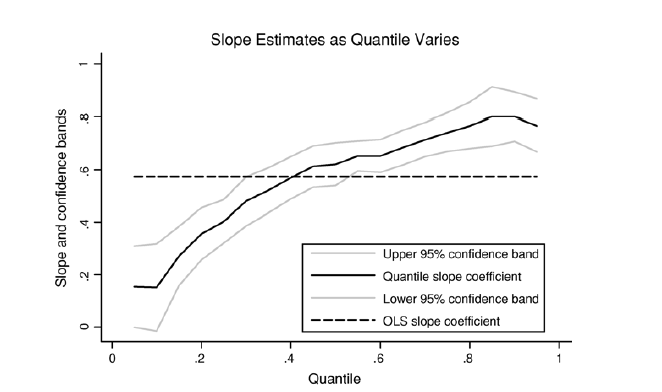
\includegraphics[keepaspectratio, width=0.8\textwidth]{qr_vietnam.png}
\end{figure}
\end{example}
\end{mdframed}

\section{Nonparametric Regression Models}
Consider a setting where we observe the data $(y_i,x_i)$ which is i.i.d. and drawn from a DGP $P_0(y|X)$. Unlike in the parametric setup, we are interested in backing out the whole or part of the data generating process $P_0(y|X)$ \textbf{without any modeling assumptions}. Specifically, back when we imposed a linear DGP, our modeling assumption is $E[y|X]=X\beta$, i.e. a linear conditional expectations. Now, we are moving away from linearity assumption by just specifying $E[y|X]=m(X)$, i.e. conditional expectation of $y$ is some function (not necessarily linear) of $X$. In essence, we are interested in an estimation problem involving an unknown function. This approach is called a \textbf{nonparametric} approach. We normally use nonparametric approach to conduct a diagnostic checking of an estimated parametric model, to conveniently display key features of the dataset in part or in whole, and to conduct an inference under very weak assumptions. \par
For discrete-valued $Y$ and $X$, this is relatively easy. We can back out the data generating process of interest
\[
\widehat{P}(y\in A| x\in B)=\frac{n^{-1}\sum_{i=1}^n\mathbb{1}(y_i\in A, x_i\in B) }{n^{-1}\sum_{i=1}^n\mathbb{1}(x_i\in B)}
\]
Provided that $P_0(x\in B)\neq 0$, then the above estimator converges to the true $P_0(y|x)$ as $n\to\infty$ almost surely.
\par
When we are working with continuous variables to get an estimate of $P_0(Y\leq y|x)$, one way we could approach is to define $A$ in the above example as $A\equiv (-\infty, y], B\equiv[x-\epsilon, x+\epsilon]$ and use $\lim_{\epsilon\to0}\widehat{P}(A|B)$ to back out the DGP. The trade-off is that as $\epsilon$ becomes smaller, there are fewer points that we can use, leading to highly volatile estimates. This is even more problematic when we have too many dimensions of $X$ (and by too many, the number required for this to happen is not that large). What we do here is to estimate the distribution with kernel density estimation. We also learn that the length of the interval is crucial, and that higher dimensions make this more difficult.
\subsection{Kernel Density Estimation} 

Consider the problem of estimating the probability density function $f(y)$ of a random scalar variable $Y$ at $Y=y$. We are putting a minimal number of restriction on what $f(y)$ could be. Let $\{y_1,...,y_n\}$ be a random sample of $Y$. One possible way to do estimate the CDF $\Pr(Y\leq y)$, if we do not control for anything, is to come up with an empirical CDF (or EDF). 

\begin{mdframed}[backgroundcolor=blue!5] 
\begin{definition}[Empirical Distribution Function] The \textbf{empirical distribution function} (or EDF) for the data $y_1,..,y_n$ is defined as
\[
F_n(y) = \frac{1}{n}\sum_{i=1}^n \mathbb{1}(y_i\leq y)
\]
\end{definition}
\end{mdframed} 
The problem with this is that EDF is a step function with range $[0,1]$ that has `jumps' at each nonzero $y_i$. Derivatives to get the pdf is tricky (a Dirac mass, or a spike) and give 0. So EDF is not useful here. 

An alternative is to find an estimator for $f$ that is smooth and non-negative. This is where kernel estimation comes in. If the true $f$ is a smooth function, we can approximate $f(y)$ by
\[
f(y)\simeq \frac{\int_{y-h}^{y+h}f(u)du}{2h}
\]
for a small $h$ (which will later be our bandwidth). The numerator on the right hand side can be estimated using a sample analogue of the following form
\[
\frac{1}{n}\sum_{i=1}^n \mathbb{1}\{y-h\leq y_i \leq y+h \}
\]
Combining the two expressions, we can approximate $f(x)$ with
\footnotesize{\begin{align*}
\hat{f}_n(y)&=\frac{n^{-1}\sum_{i=1}^n \mathbb{1}[y-h\leq y_i \leq y+h]}{2h} \\
&=\frac{1}{2nh}\sum_{i=1}^n \mathbb{1}[y-h\leq y_i \leq y+h]\\
&=\frac{1}{nh}\sum_{i=1}^n \frac{1}{2}\mathbb{1}\left[\left|\frac{y-y_i}{h}\right| \leq 1\right]\\
&=\frac{1}{nh}\sum_{i=1}^n K\left(\frac{y-y_i}{h}\right)\\
&=\frac{1}{n}\sum_{i=1}^n K_h(y-y_i)
\end{align*}}\normalsize
where $K(u)=\frac{1}{2}1(|u|\leq 1)$ and $K_h = \frac{1}{h}K\left(\frac{\cdot}{h}\right)$. $\hat{f}_n(y)$ is a \textbf{kernel density estimator} for $f(y)$. Specifically for this example, I have used a uniform kernel because this is very simple for discussion and derivation. \par
Notable property of the kernel estimator is that it shares the properties with the kernel $K$ we choose. They are smooth, positive (or at least non-negative), and integrates to 1 over the domain. This is something that we do not get with just an EDF.  \par
As for the type of kernel density estimators, there can be many. The requirements are that $K$ is a real-to-real function, positive and smooth and integrates to 1 on its support. For instance, you can use a Gaussian Kernel, triangular kernel or an Epanechinkov kernel, defined as $K(u)=\frac{3}{4}\max\{1-u^2,0\}$. However, the selection of $K$ does not matter in most cases. 

 \begin{mdframed}[backgroundcolor=yellow!5]
\begin{comment}[Types of kernel]
Here are the famous kernels in use. The Stata default is Epanechnikov kernel. 
\begin{figure}[H]
\centering
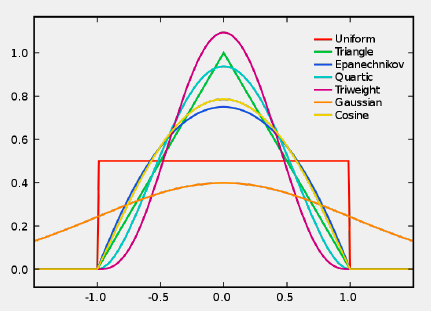
\includegraphics[width=0.67\textwidth, keepaspectratio]{kernel.png}
\end{figure}
\end{comment}
\end{mdframed}
\subsection{Choice of the bandwidth $h$}
While we may have some freedom in choosing $K$, same cannot be said for the bandwidth $h$. This is because our choice of $h$ directly affects the trade-off between the bias and the variance. A simple, descriptive way to see why it matters is to check that small bandwidth leads to undersmoothing and large bandwidth leads to oversmoothing.

 \begin{mdframed}[backgroundcolor=yellow!5]
\begin{comment}[So why worry about bandwidth to begin with?]
If $h$ is smaller than the optimal bandwidth length, we say that there is an \textbf{undersmoothing}. If otherwise, we say \textbf{oversmoothing} is present. When there is an undersmoothing, there are too much more detail than necessary and in some areas, leading to computational difficulty. When there is an oversmoothing, we risk masking some important detail about the distribution of $f(x)$. We may end up with a normal distribution even if it really is not. \par
Below is a figure that I borrowed from a statistics lecture note from CMU.\footnote{https://www.stat.cmu.edu/~larry/=sml/densityestimation.pdf} (called Bart Simpson graph)
\begin{figure}[H]
\centering
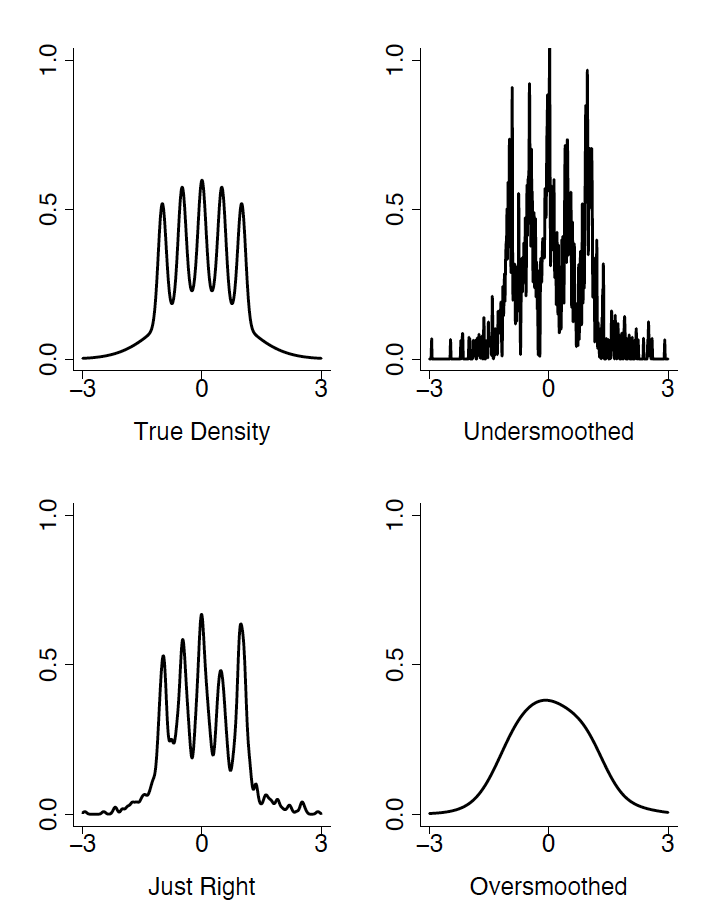
\includegraphics[width=0.5\textwidth, keepaspectratio]{smoothing.png}
\end{figure}
\end{comment}
\end{mdframed}
\par
Rigorously speaking, the problem underlying this trade-off is the bias-variance tradeoff. This is really something that we did not worry as much in parametric setting since increasing $n$ solves all the problem by reducing bias and variance. To see this, we can break down the mean squared error into 
\[
\begin{aligned}
E[(\hat{\theta}-\theta)^2]&=E[((\hat{\theta}-E[\hat{\theta}])+(E[\hat{\theta}]-\theta))^2]\\
&=E[(\hat{\theta}-E[\hat{\theta}])^2+(E[\hat{\theta}]-\theta)^2+2(\hat{\theta}-E[\hat{\theta}])(E[\hat{\theta}]-\theta)]\\
&=E[(\hat{\theta}-E[\hat{\theta}])^2]+E[(E[\hat{\theta}]-\theta)^2]+2E[(\hat{\theta}-E[\hat{\theta}])(E[\hat{\theta}]-\theta)]\\
&=\underbrace{E[(\hat{\theta}-E[\hat{\theta}])^2]}_{V(\hat{\theta})}+\underbrace{(E[\hat{\theta}]-\theta)^2}_{\text{Bias}(\hat{\theta},\theta)^2}
\end{aligned}
\]
It can be shown that bias is $O\left(\frac{1}{n^2}\right)$ and that variance is $O\left(\frac{1}{n}\right)$ so increasing $n$ reduces both. 
\par
In nonparametrics, this is tricky since we also need to worry about $h$. When we are calculating bias and variance for the kernel estimators, $h$ plays not just an important role but also a contrasting role in determining the bias and variance. 
To see this, we first formulate the bias of the estimate of $f(y)$.
\footnotesize{\begin{align*}
E[\hat{f}_n(y)]&=E\left[\frac{1}{nh}\sum_{i=1}^n K\left(\frac{y-y_i}{h}\right)\right]\\
&=\frac{1}{h}\int_{-\infty}^\infty K\left(\frac{y-t}{h}\right)f(t)dt\\
&=\frac{1}{h}\int_{-\infty}^\infty K(-u)f(y+uh)(hdu) \ \left(\because \frac{t-y}{h}=u \ \text{transformation, also } du=\frac{1}{h}dt\right)\\
&=\int_{-\infty}^\infty K(-u)f(y+uh)du\\
&=\int_{-\infty}^\infty K(-u)\left[f(y)+f'(y)uh + \frac{f''(y)u^2h^2}{2}+o(h^2)\right]dt \ (\because \text{Taylor approximate around $y$}) \\
&=f(y)+0+\frac{1}{2}\int_{-\infty}^\infty K(-u)u^2h^2f''(y)du + o(h^2)
\end{align*}}\normalsize
Where $\int_{-\infty}^\infty K(-u)du=\int_{-\infty}^\infty K(u)du=1$ by symmetry of the kernel estimator and that it integrates to 1. This  produces $f(y)$. Also, $\int_{-\infty}^\infty uK(u)dt=0$ (since kernel is symmetric around 0) justifies second term in the last line being 0. You can also flip the signs in $K(\cdot)$ because of symmetry. As such, the bias is captured by 
\[
E[\hat{f}(x)]-f(x)=\frac{1}{2}\int_{-\infty}^\infty K(u)u^2h^2f''(y)du
\]
Therefore, smaller bandwidth $h$ reduces the bias.\par
However, for variance, we have
 \footnotesize{\begin{align*}
Var[\hat{f}_n(y)]&=E[\hat{f}^2(y)]-(E[\hat{f}(y)])^2\\ 
&=E\left[\frac{1}{n^2h^2}\left(\sum_{i=1}^nK\left(\frac{y-y_i}{h}\right)\right)^2\right]-(E[\hat{f}(y)])^2\\
&=E\left[\frac{1}{n^2h^2}\left(\sum_{i=1}^nK^2\left(\frac{y-y_i}{h}\right)+2\sum_{i<j} K\left(\frac{y-y_i}{h}\right)K\left(\frac{y-y_j}{h}\right)\right)\right]-(E[\hat{f}(y)])^2\\
&=\frac{1}{nh^2}\int_{-\infty}^\infty K^2\left(\frac{y-t}{h}\right)f(t)dt+\frac{n(n-1)}{n^2h^2}\left(\int_{-\infty}^\infty K\left(\frac{y-t}{h}\right)f(t)dt\right)^2-\frac{1}{h^2}\left(\int_{-\infty}^\infty K\left(\frac{y-t}{h}\right)f(t)dt\right)^2
 \end{align*}}\normalsize
 Then, we use the Taylor expansion and the variable transformation $\frac{t-y}{h}=u$ on each of the terms. As a result, we can show that the first term can be written
  \footnotesize{\[
 \frac{1}{nh^2}\int_{-\infty}^\infty K^2\left(\frac{y-t}{h}\right)f(t)dt=\frac{1}{nh}\int_{-\infty}^\infty K^2(-u)f(y+uh)du\simeq \frac{1}{nh}\int_{-\infty}^\infty K^2(u)f(y)du
 \]}\normalsize
 So  $\frac{1}{nh}\int_{-\infty}^\infty K^2(u)f(y)du$ is the leading term. \par
 The other two terms will be cancelled out as $n\to\infty$, as 
 \footnotesize{\[
\left( \frac{n(n-1)}{n^2h^2}-\frac{1}{h^2}\right)\left(\int_{-\infty}^\infty K\left(\frac{y-t}{h}\right)f(t)dt\right)^2 =-\frac{1}{nh^2} \left(\int_{-\infty}^\infty K\left(\frac{y-t}{h}\right)f(t)dt\right)^2
 \]}\normalsize
   Since the first term can be written as $O\left(\frac{1}{nh}\right)$, the remaining two terms are dominated (since they have $h^2$) and smaller $h$ increases the variance.  \par
   So what determines the optimal $h$? The answer is the $h$ that minimizes the loss function, or asymptotic mean integrated squared error (AMISE), defined as
 \[
 \int E[\hat{f}_n(y)-f(y)]^2dy
 \]
 where the bias-variance decomposition of MSE kicks in as follows
 \small{\begin{align*}
 E[(\hat{f}_n(y)-f(y))^2] &=E[(\hat{f}_n(y)-E[\hat{f}_n(y)]+E[\hat{f}_n(y))-f(y)]^2]\\
 &=E[(\hat{f}_n(y)-E[\hat{f}_n(y)])^2+(E[\hat{f}_n(y)]-f(y))^2 +2(\hat{f}_n(y)-E[\hat{f}_n(y)])(E[\hat{f}_n(y)]-f(y))]\\
 &=E[(\hat{f}_n(y)-E[\hat{f}_n(y)])^2]+E[(E[\hat{f}_n(y)]-f(y))^2]\\
  &=\underbrace{E[(\hat{f}_n(y)-E[\hat{f}_n(y)])^2]}_{V(\hat{f}_n)(y)}+\underbrace{(E[\hat{f}_n(y)]-f(y))^2}_{\text{Bias}(\hat{f}_n(y), f(y))^2}\\
 \end{align*}}\normalsize\par
  From the discussion about the bias and variance above, we can write
   \begin{align*}
 E[(\hat{f}_n(y)-f(y))^2] =\frac{1}{nh}\int_{-\infty}^\infty K^2(u)f(y)du+\frac{h^4}{4}(f''(y))^2\left(\int_{-\infty}^\infty K(u)u^2du\right)^2
 \end{align*}
 Thus, the final version of AMISE can be written as
 \[
 \int(\text{Variance}+\text{Bias}^2)dy=\frac{1}{nh}\int_{-\infty}^\infty K^2(u)du+\frac{h^4}{4}\int_{-\infty}^\infty(f''(y))^2\left(\int_{-\infty}^\infty K(u)u^2du\right)^2 dy
 \]
 For a shorthand notation, we can write $A=\frac{1}{4}\int_{-\infty}^\infty(f''(y))^2\left(\int_{-\infty}^\infty K(u)u^2du\right)^2 dy$, and let $B=\int_{-\infty}^\infty K^2(u)du$ to get
 \[
 AMISE =Ah^4+\frac{B}{nh}
 \]
Then, the minimization problem becomes $\min_h AMISE$. Therefore, we find $h$ satisfying
 \[
 4Ah^3-Bn^{-1}h^{-2}=0\iff h^5=\frac{B}{4An} \iff h=\left(\frac{B}{4An}\right)^{1/5}
 \]
 In this framework, the bias and standard errors are both in $n^{-2/5}$ and AMISE will be in $n^{-4/5}$. Therefore, we may not have a CAN estimator at $n^{-1/2}$, which is what is normally the case. Even bigger problem arises from $\int f''(x)dx$ term in $A$, as we are not sure of $f(x)$ to begin with, we do not know what $f''(x)$ would be. There are several ways to deal with this.
 \begin{itemize}
 \item\textbf{Silverman's Rule of Thumb}: If $K$ is a normal kernel and $f(y)$ is normal with some variance $\sigma^2$, Silverman's rule of thumb implies the benchmark
 \[
 h=1.06\sigma n^{-1/5}
 \]
 where $\sigma$ can be replaced with sample standard deviation $s$. For a more robust version, we can use
 \[
 h=0.9 \min\{s,IQ/1.34\}n^{-1/5}
 \]
 where $IQ$ is an interquartile distance. 
 \item\textbf{Cross-validation}: This method is similar to the original method in the sense that we are selecting some $h$ that minimizes certain criterion function, $CV(h)$. In this case, we are using a leave-one-out estimator. This is usually calculated as
 \[
 \hat{f}_{-i}(y) = \frac{1}{nh}\sum_{j\neq i}K\left(\frac{y-y_j}{h}\right)
 \]
 for every observation $i$. This is computationally burdensome and the resulting $h$ converges very slowly ($n^{-1/10}$). 
  \item\textbf{Local Bandwidth}: You may care only about $f(y)$ at a given point. The key idea is to make $h$ larger in a low density area, as low density could imply larger spread in the distribution of $f(y)$. Making $h$ larger would decrease variance. In a wiggly region, it is better to take $h$ smaller. The distribution can take many values and bias can be problematic. Reducing $h$ would minimize worries about biases. 
 \end{itemize}

 
%%%%%%%%%%%%%%%
\end{document}

